\providecommand{\main}{../../..}
\documentclass[\main/dresen_thesis.tex]{subfiles}

\begin{document}
  \section{Grazing-Incidence Small-Angle Neutron Scattering (GISANS)}
    \label{ch:methods:gisans}
    The GISANS and polGISANS experiment is basically analogue to GISAXS with the same modifications that have been done when going from SAXS to SANS and SANSPOL.
    Meaning, similarly to GISAXS a sample is placed in a neutron beam at a small angle close to the critical angle of the sample and the integrated intensity is measured on a position-sensitive detector, where the coordinate transformation from pixel coordinates to $q$-space is analogue.
    For polGISANS, two measurements are performed on a magnetic sample for the two polarization states of the neutrons, as in SANSPOL.
    Additionally, as the magnetic state of a sample is studied, it is of interest to measure at low temperatures to minimize thermal averaging in the magnetization.

    \begin{figure}[tb]
      \centering
      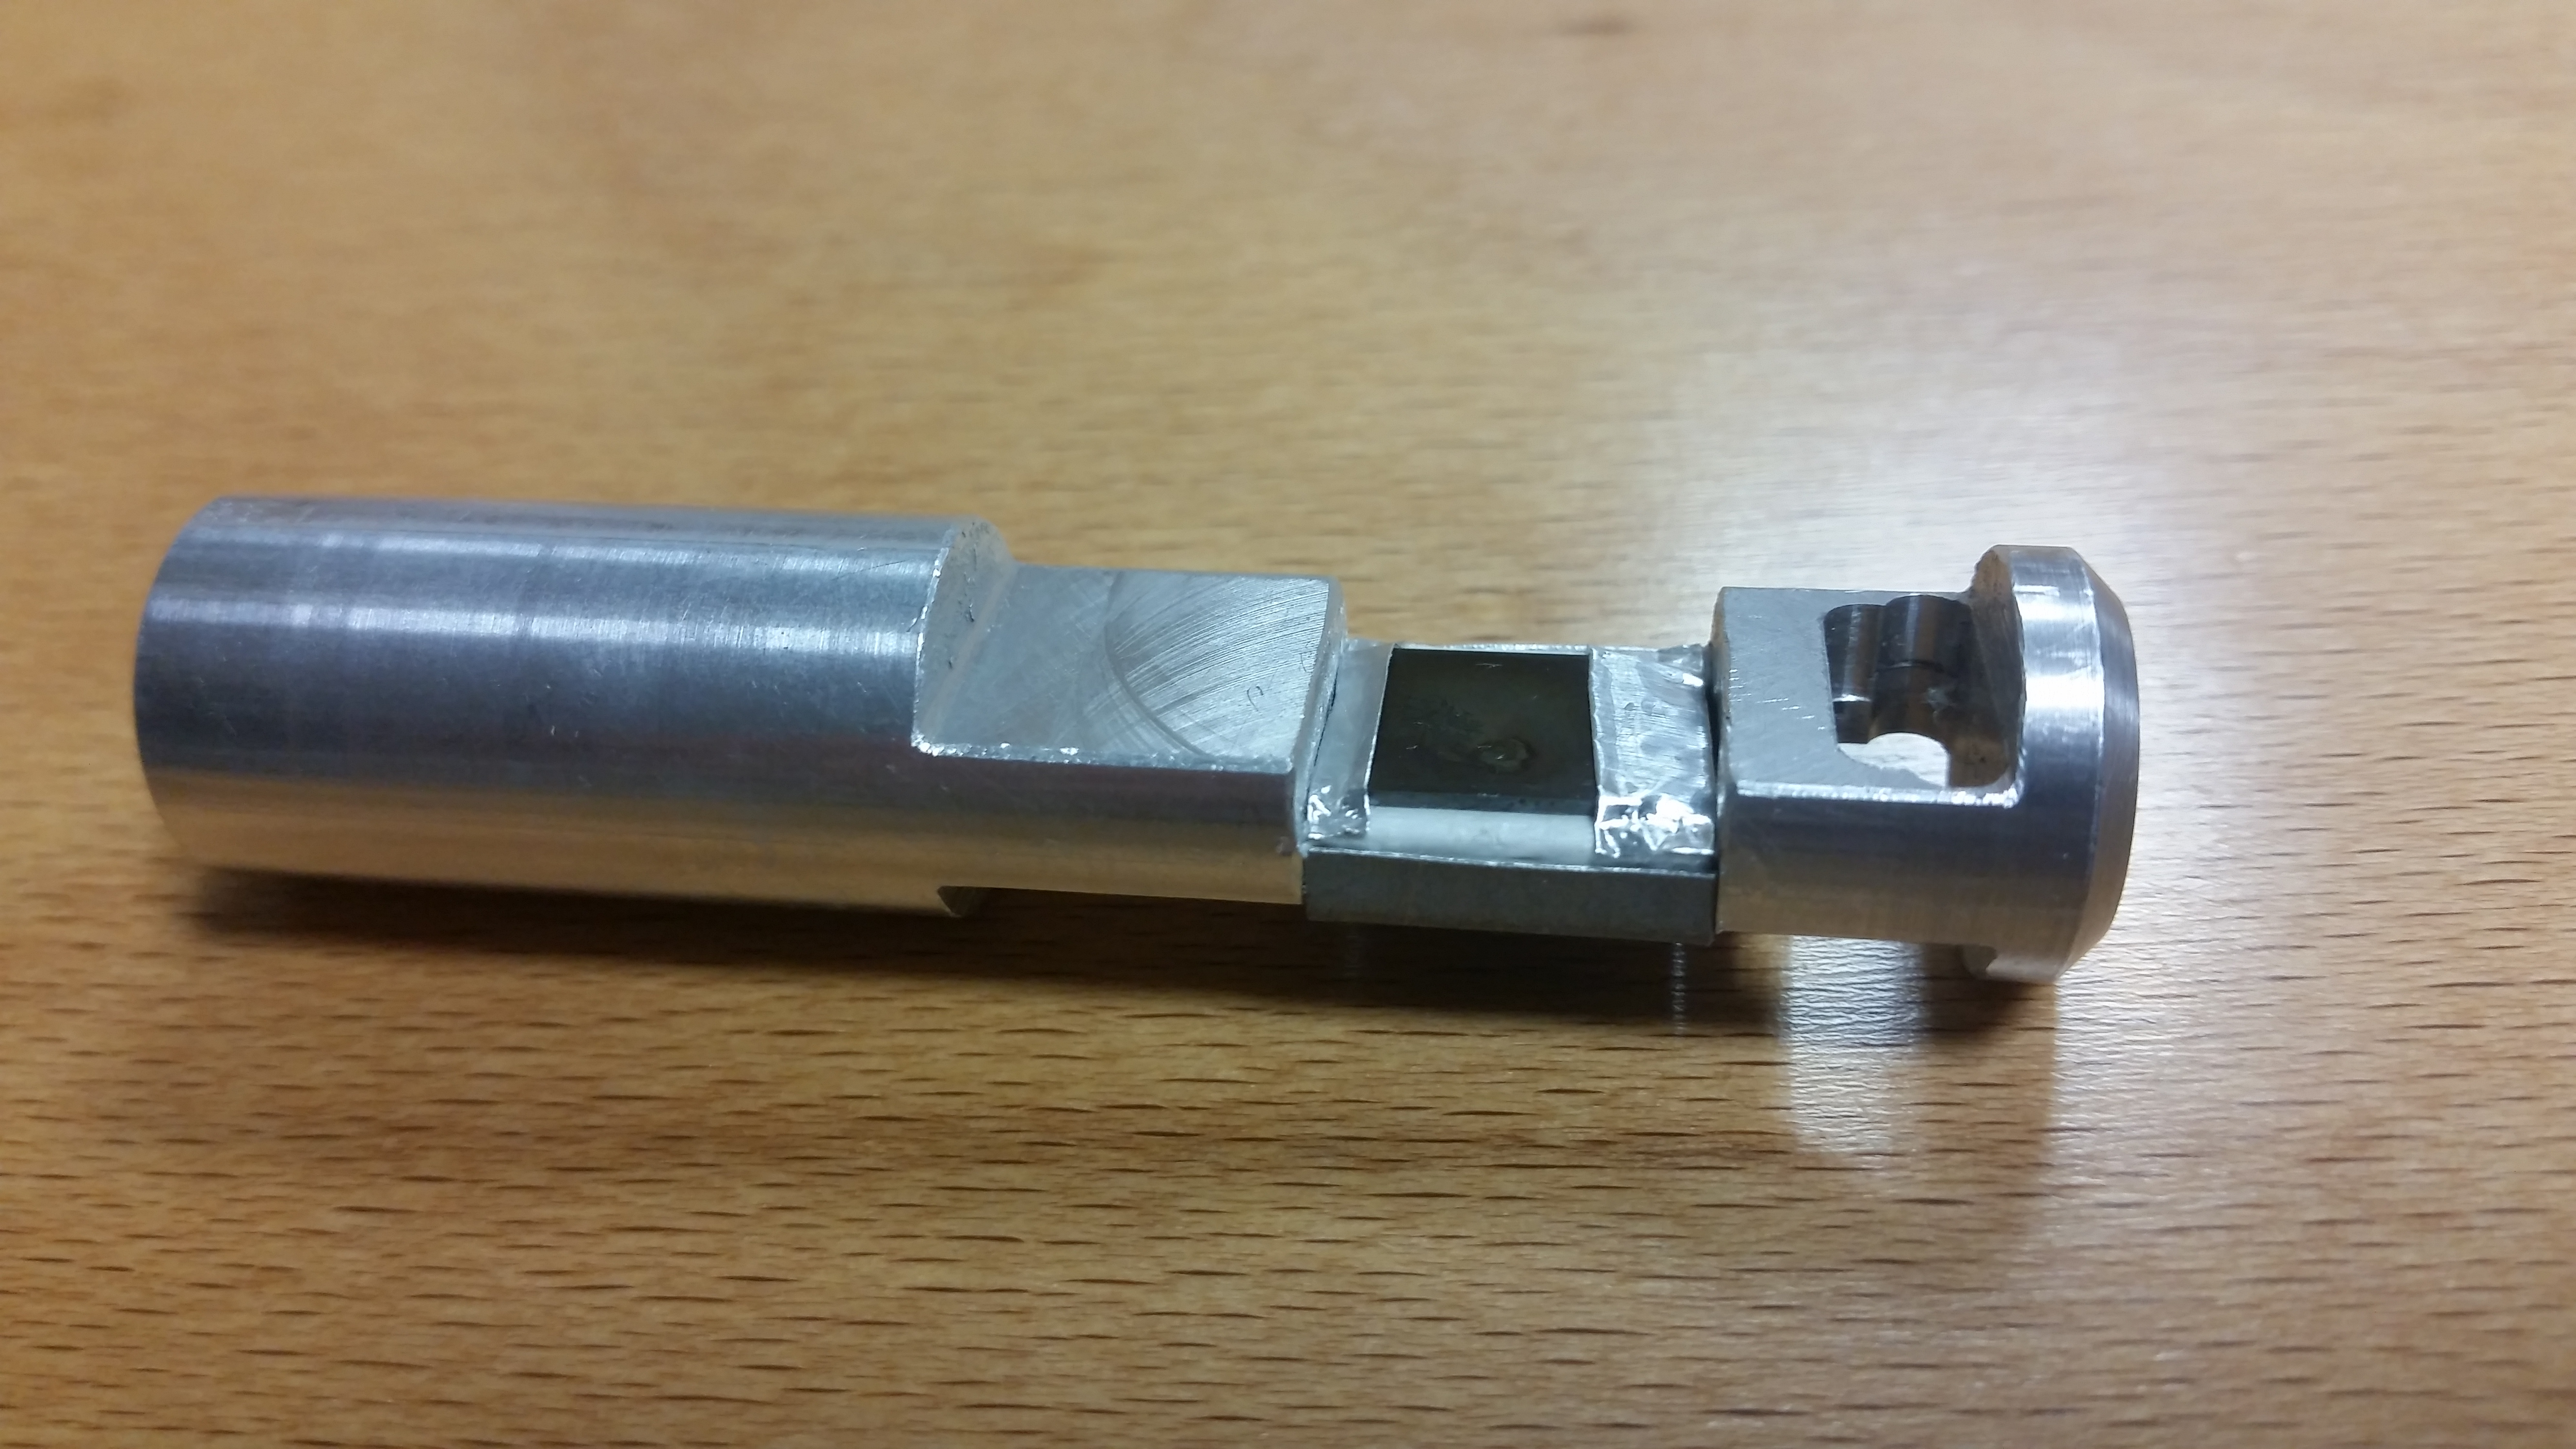
\includegraphics[width=0.7\textwidth]{appendix_methods_gisans_sample}
      \caption{\label{fig:methods:gisans:samples}In the GISANS experiment, the sample is mounted with sticky tape and aluminium foil on an screwable aluminium holder. To minimize the scattering from the holder and the sticky tape, cadmium stripes are attached on the side below the sample.}
    \end{figure}

    For this purpose, the sample needs is placed in a cryo-magnet, which allows to reduce the temperature to the Helium level and apply magnetic fields.
    For this purpose the sample is typically mounted on a screwable aluminium holder as shown in \reffig{fig:methods:gisans:samples}, such that it can be fixed on a rod and lowered into a cryo-magnet.
    As the sample is hanging in this geometry, it is fixed tightly with sticky tape and aluminium foil to ensure that it does not move during the measurement.
    The sticky tape is covered with cadmium to minimize the incoherent scattering coming from the sample holder.

    All presented GISANS experiments in this thesis have been performed on the D33 instrument at ILL \refapp{ch:lss:d33}.
    Meaning that the MATLAB script GRASP can be used to analyze the data and perform line cuts and integrations as in SANS.
    Due to better stability and easier handling to the MATLAB framework, it was however preferred to perform the analysis of the data in the Python programming language by loading the NeXus data format into memory with the package h5py \cite{collette_2013_h5py} and using NumPy for the data treatment \cite{Oliphant_2006_Guide}.

    For the model calculations the BornAgain software package is used, which allows to additionally define magnetic scattering length densities, as well as the polarization of incoming neutrons.
\end{document}